% Chapter 4
\chapter{روش پیشنهادی}

%%%%%%%%%%%%%%%%%%%%%%%%%%%%%%%
%%%%%%%%%%%%%%%%%%%%%%%%%%%%%%%
\section{شرح مسئله}
همانطورکه پیش‌تر بیان‌شد، یکی از نقاط ضعف Modex مربوط به عدم فراخوانی هیچ گونه رویه ای است. این موجب می‌شود تا تبدیل توابع کد C به رویه ها در کد Promela ، در برخی کدهای پیچیده‌تر با مشکل جدی مواجه شود. برای مثال، در برنامه‌های با فراخوانی‌های پیچیده‌تر توابع در زبان C ، ترتیب اجرای رویه های کد Promela تولید شده، مطابق با ترتیب اجرای صحیح توابع کد C اولیه نخواهدبود. برای درک بهتر مسئله، در ادامه با بیان یک مثال، این مشکل شرح داده‌خواهدشد و راه حلی با تمرکز بر روی همین مثال ارائه خواهدشد.
شکل 4-1 که کد به زبان C را نشان می‌دهد، در نظر بگیرید.

 \begin{figure}
	\centering
	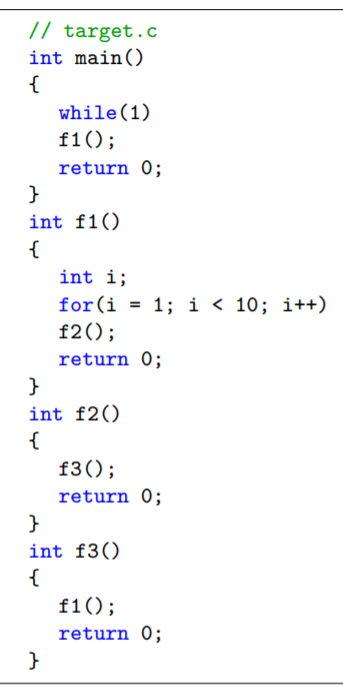
\includegraphics[height=10cm,width=6cm]{b.png}
	\caption{کد به زبان C}
	\centering
\end{figure}


%\hspace{0.5cm}
%\begin{latin}
%\begin{lstlisting}
%	// target.c
%	int main()
%	{
%		while(1)
%		f1();
%		return 0;
%	}
%	int f1()
%	{
%		int i;
%		for(i = 1; i < 10; i++)
%		f2();
%		return 0;
%	}
%	int f2()
%	{
%		f3();
%		return 0;
%	}
%	int f3()
%	{
%		f1();
%		return 0;
%	}
%\end{lstlisting}
%\end{latin}


\section{مدل سازی با Modex}
می خواهیم این کد را به Promela  ترجمه کنیم،
\subsection{حالت اول}
اگر فایل \lr{target.prx} نداشته باشیم(یا این فایل خالی باشد)، و یا اینکه محتوای آن مانند کد نشان داده شده در شکل 4-2 باشد، کد Promela تولید شده توسط Modex ، به صورت کد نشان داده شده در دو شکل 4-3 و 4-4 خواهدبود.

 \begin{figure}
	\centering
	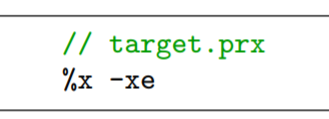
\includegraphics[height=1.5cm,width=4cm]{c.png}
	\caption{محتوای فایل .prx}
	\centering
\end{figure}

% \hspace{0.5cm}
% \begin{latin}
% 	\begin{lstlisting}
% 		// target.prx
% 		%x -xe
% 	\end{lstlisting}
% \end{latin}


 \begin{figure}
	\centering
	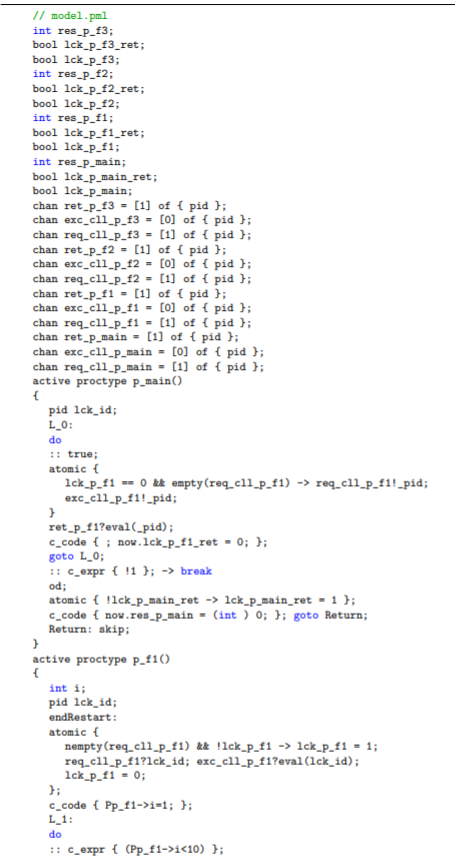
\includegraphics[height=25cm,width=12cm]{d1.png}
	\caption{فایل نتیجه Modex}
	\centering
\end{figure}

 \begin{figure}
	\centering
	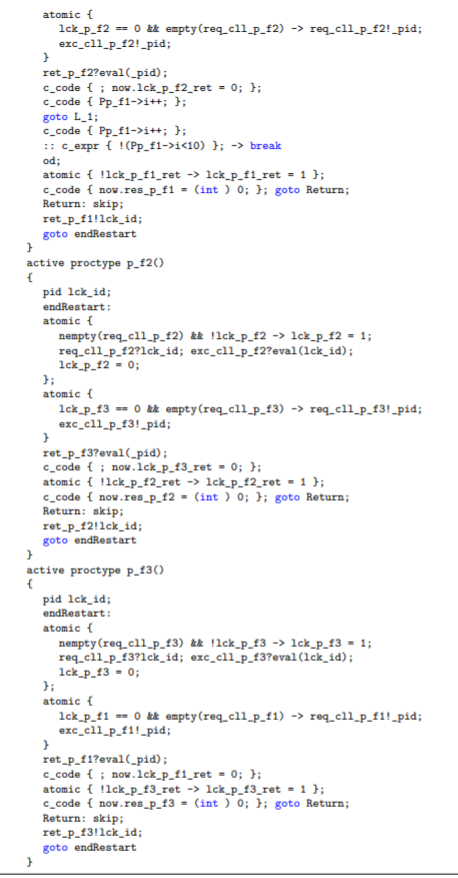
\includegraphics[height=25cm,width=12cm]{d2.png}
	\caption{ادامه فایل نتیجه Modex}
	\centering
\end{figure}

%\hspace{0.5cm}
%\begin{latin}
%	\begin{lstlisting}
%		// model.pml
%		int res_p_f3;
%		bool lck_p_f3_ret;
%		bool lck_p_f3;
%		int res_p_f2;
%		bool lck_p_f2_ret;
%		bool lck_p_f2;
%		int res_p_f1;
%		bool lck_p_f1_ret;
%		bool lck_p_f1;
%		int res_p_main;
%		bool lck_p_main_ret;
%		bool lck_p_main;
%		chan ret_p_f3 = [1] of { pid };
%		chan exc_cll_p_f3 = [0] of { pid };
%		chan req_cll_p_f3 = [1] of { pid };
%		chan ret_p_f2 = [1] of { pid };
%		chan exc_cll_p_f2 = [0] of { pid };
%		chan req_cll_p_f2 = [1] of { pid };
%		chan ret_p_f1 = [1] of { pid };
%		chan exc_cll_p_f1 = [0] of { pid };
%		chan req_cll_p_f1 = [1] of { pid };
%		chan ret_p_main = [1] of { pid };
%		chan exc_cll_p_main = [0] of { pid };
%		chan req_cll_p_main = [1] of { pid };
%		active proctype p_main()
%		{
%			pid lck_id;
%			L_0:
%			do
%			:: true;
%			atomic {
%				lck_p_f1 == 0 && empty(req_cll_p_f1) -> req_cll_p_f1!_pid;
%				exc_cll_p_f1!_pid;
%			}
%			ret_p_f1?eval(_pid);
%			c_code { ; now.lck_p_f1_ret = 0; };
%			goto L_0;
%			:: c_expr { !1 }; -> break
%			od;
%			atomic { !lck_p_main_ret -> lck_p_main_ret = 1 };
%			c_code { now.res_p_main = (int ) 0; }; goto Return;
%			Return: skip;
%		}
%		active proctype p_f1()
%		{
%			int i;
%			pid lck_id;
%			endRestart:
%			atomic {
%				nempty(req_cll_p_f1) && !lck_p_f1 -> lck_p_f1 = 1;
%				req_cll_p_f1?lck_id; exc_cll_p_f1?eval(lck_id);
%				lck_p_f1 = 0;
%			};
%			c_code { Pp_f1->i=1; };
%			L_1:
%			do
%			:: c_expr { (Pp_f1->i<10) };
%			atomic {
%				lck_p_f2 == 0 && empty(req_cll_p_f2) -> req_cll_p_f2!_pid;
%				exc_cll_p_f2!_pid;
%			}
%			ret_p_f2?eval(_pid);
%			c_code { ; now.lck_p_f2_ret = 0; };
%			c_code { Pp_f1->i++; };
%			goto L_1;
%			c_code { Pp_f1->i++; };
%			:: c_expr { !(Pp_f1->i<10) }; -> break
%			od;
%			atomic { !lck_p_f1_ret -> lck_p_f1_ret = 1 };
%			c_code { now.res_p_f1 = (int ) 0; }; goto Return;
%			Return: skip;
%			ret_p_f1!lck_id;
%			goto endRestart
%		}
%		active proctype p_f2()
%		{
%			pid lck_id;
%			endRestart:
%			atomic {
%				nempty(req_cll_p_f2) && !lck_p_f2 -> lck_p_f2 = 1;
%				req_cll_p_f2?lck_id; exc_cll_p_f2?eval(lck_id);
%				lck_p_f2 = 0;
%			};
%			atomic {
%				lck_p_f3 == 0 && empty(req_cll_p_f3) -> req_cll_p_f3!_pid;
%				exc_cll_p_f3!_pid;
%			}
%			ret_p_f3?eval(_pid);
%			c_code { ; now.lck_p_f3_ret = 0; };
%			atomic { !lck_p_f2_ret -> lck_p_f2_ret = 1 };
%			c_code { now.res_p_f2 = (int ) 0; }; goto Return;
%			Return: skip;
%			ret_p_f2!lck_id;
%			goto endRestart
%		}
%		active proctype p_f3()
%		{
%			pid lck_id;
%			endRestart:
%			atomic {
%				nempty(req_cll_p_f3) && !lck_p_f3 -> lck_p_f3 = 1;
%				req_cll_p_f3?lck_id; exc_cll_p_f3?eval(lck_id);
%				lck_p_f3 = 0;
%			};
%			atomic {
%				lck_p_f1 == 0 && empty(req_cll_p_f1) -> req_cll_p_f1!_pid;
%				exc_cll_p_f1!_pid;
%			}
%			ret_p_f1?eval(_pid);
%			c_code { ; now.lck_p_f1_ret = 0; };
%			atomic { !lck_p_f3_ret -> lck_p_f3_ret = 1 };
%			c_code { now.res_p_f3 = (int ) 0; }; goto Return;
%			Return: skip;
%			ret_p_f3!lck_id;
%			goto endRestart
%		}
%	\end{lstlisting}
%\end{latin}

حال برای بررسی این مدل و مسیرهای اجرایی ممکن در آن، از Spin استفاده می‌کنیم.
\\
به طور کلی 5 مسیر اجرایی ممکن به شرح زیر برای مدل تولید شده، محتمل است:

\begin{enumerate}
	\item به ترتیب از راست به چپ main ، f1  ، f2  و درنهایت f3 اجرا می‌‌شود. و برنامه به اتمام می‌رسد.
	\item به ترتیب از راست به چپ main ، f1  ،  main ، f1  ، f2  و درنهایت f3 اجرا می‌‌شود. و برنامه به اتمام می‌رسد.
	\item به ترتیب از راست به چپ main ، f1  ،  main ، و درنهایت f1 اجرا می‌‌شود. و برنامه به اتمام می‌رسد.
	\item به ترتیب از راست به چپ main ، f1  ، و درنهایت main اجرا می‌‌شود. و برنامه به اتمام می‌رسد.
	\item فقط main اجرا می‌‌شود. و برنامه به اتمام می‌رسد.
\end{enumerate}
برای مثال، مسیر اجرایی چهارم به صورت شکل 4-5 است:

 \begin{figure}
	\centering
	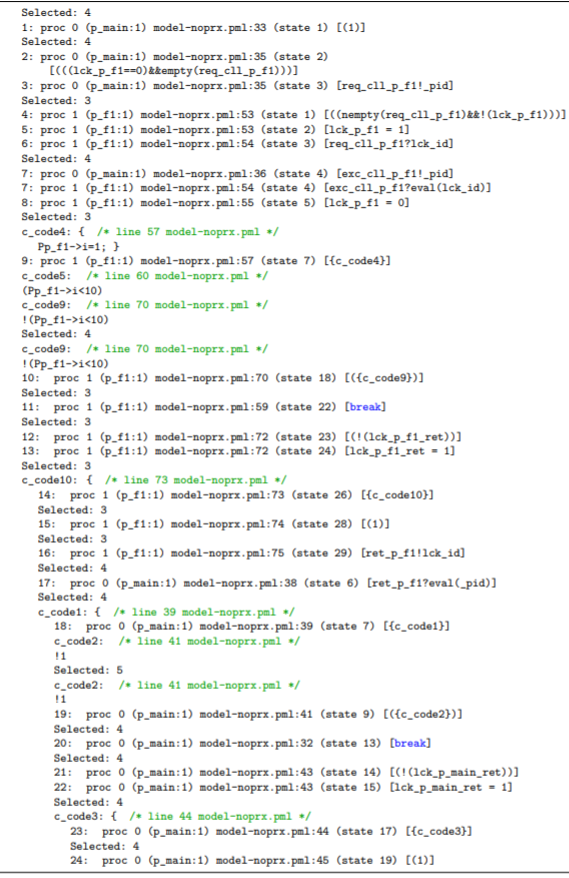
\includegraphics[height=25cm,width=16cm]{e.png}
	\caption{مسیر اجرایی}
	\centering
\end{figure}

%\begin{latin}
%	\begin{lstlisting}
%	Selected: 4
%	1:	proc  0 (p_main:1) model-noprx.pml:33 (state 1)	[(1)]
%	Selected: 4
%	2:	proc  0 (p_main:1) model-noprx.pml:35 (state 2)	[(((lck_p_f1==0)&&empty(req_cll_p_f1)))]
%	3:	proc  0 (p_main:1) model-noprx.pml:35 (state 3)	[req_cll_p_f1!_pid]
%	Selected: 3
%	4:	proc  1 (p_f1:1) model-noprx.pml:53 (state 1)	[((nempty(req_cll_p_f1)&&!(lck_p_f1)))]
%	5:	proc  1 (p_f1:1) model-noprx.pml:53 (state 2)	[lck_p_f1 = 1]
%	6:	proc  1 (p_f1:1) model-noprx.pml:54 (state 3)	[req_cll_p_f1?lck_id]
%	Selected: 4
%	7:	proc  0 (p_main:1) model-noprx.pml:36 (state 4)	[exc_cll_p_f1!_pid]
%	7:	proc  1 (p_f1:1) model-noprx.pml:54 (state 4)	[exc_cll_p_f1?eval(lck_id)]
%	8:	proc  1 (p_f1:1) model-noprx.pml:55 (state 5)	[lck_p_f1 = 0]
%	Selected: 3
%	c_code4:	{ 	/* line 57 model-noprx.pml */
%		Pp_f1->i=1;  }
%	9:	proc  1 (p_f1:1) model-noprx.pml:57 (state 7)	[{c_code4}]
%	c_code5:		/* line 60 model-noprx.pml */
%	(Pp_f1->i<10) 
%	c_code9:		/* line 70 model-noprx.pml */
%	!(Pp_f1->i<10) 
%	Selected: 4
%	c_code9:		/* line 70 model-noprx.pml */
%	!(Pp_f1->i<10) 
%	10:	proc  1 (p_f1:1) model-noprx.pml:70 (state 18)	[({c_code9})]
%	Selected: 3
%	11:	proc  1 (p_f1:1) model-noprx.pml:59 (state 22)	[break]
%	Selected: 3
%	12:	proc  1 (p_f1:1) model-noprx.pml:72 (state 23)	[(!(lck_p_f1_ret))]
%	13:	proc  1 (p_f1:1) model-noprx.pml:72 (state 24)	[lck_p_f1_ret = 1]
%	Selected: 3
%	c_code10:	{ 	/* line 73 model-noprx.pml */
%	14:	proc  1 (p_f1:1) model-noprx.pml:73 (state 26)	[{c_code10}]
%	Selected: 3
%	15:	proc  1 (p_f1:1) model-noprx.pml:74 (state 28)	[(1)]
%	Selected: 3
%	16:	proc  1 (p_f1:1) model-noprx.pml:75 (state 29)	[ret_p_f1!lck_id]
%	Selected: 4
%	17:	proc  0 (p_main:1) model-noprx.pml:38 (state 6)	[ret_p_f1?eval(_pid)]
%	Selected: 4
%	c_code1:	{ 	/* line 39 model-noprx.pml */
%	18:	proc  0 (p_main:1) model-noprx.pml:39 (state 7)	[{c_code1}]
%	c_code2:		/* line 41 model-noprx.pml */
%	!1 
%	Selected: 5
%	c_code2:		/* line 41 model-noprx.pml */
%	!1 
%	19:	proc  0 (p_main:1) model-noprx.pml:41 (state 9)	[({c_code2})]
%	Selected: 4
%	20:	proc  0 (p_main:1) model-noprx.pml:32 (state 13)	[break]
%	Selected: 4
%	21:	proc  0 (p_main:1) model-noprx.pml:43 (state 14)	[(!(lck_p_main_ret))]
%	22:	proc  0 (p_main:1) model-noprx.pml:43 (state 15)	[lck_p_main_ret = 1]
%	Selected: 4
%	c_code3:	{ 	/* line 44 model-noprx.pml */
%	23:	proc  0 (p_main:1) model-noprx.pml:44 (state 17)	[{c_code3}]
%	Selected: 4
%	24:	proc  0 (p_main:1) model-noprx.pml:45 (state 19)	[(1)]
%	\end{lstlisting}
%\end{latin}

اگر به برنامه C موردنظر توجه کنید، متوجه می‌شوید که این برنامه در تابع اصلی (main) دارای یک حلقه‌ی بی‌نهایت است و منطقاً نباید هیچ‌گاه فراخوانی توابع به پایان برسد. ولی در مدل Promela تولید شده، در همه‌ی حالت‌ها فراخوانی توابع تمام می‌شود و مدل‌سازی به پایان می‌رسد.
\\
حالا اگر به مدل Promela تولید شده توجه کنید، متوجه می‌شوید که این اتمام زودهنگام فراخوانی‌ها به همان دلیل عدم امکان فراخوانی رویه‌ها در کد تولیدی Modex ، که پیش‌تر عنوان شد، است. تمام رویه‌های تولید شده در این کد، به صورت فعال\LTRfootnote{active proctype}  استفاده شده‌اند و با استفاده از کانال‌های هم‌گام‌ساز \LTRfootnote{synchronization channels}   سعی شده که تا حدی ابتدایی ترتیب اجرای آن‌ها رعایت شود. ولی با توجه به اینکه رویه‌های از ابتدا فعال، فقط به صورت یک نمونه\LTRfootnote{instance}   از آن رویه عمل می‌کنند، این ساختار تولید مدل نمی‌تواند در یک شرایط پیچیده از فراخوانی رویه ها، پاسخگوی اجرای درست رویه‌ها باشد.


\subsection{حالت دوم}
اگر محتوای فایل \lr{target.prx} آن مانند کد نشان داده شده در شکل 4-6 باشد، کد Promela تولید شده توسط Modex ، به صورت کد نشان داده شده در شکل 4-7 خواهدبود.

 \begin{figure}
	\centering
	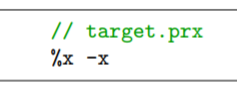
\includegraphics[height=1.5cm,width=4cm]{f.png}
	\caption{محتوای فایل .prx}
	\centering
\end{figure}


%\hspace{0.5cm}
%\begin{latin}
%	\begin{lstlisting}
%		// target.prx
%		%x -x
%	\end{lstlisting}
%\end{latin}

 \begin{figure}
	\centering
	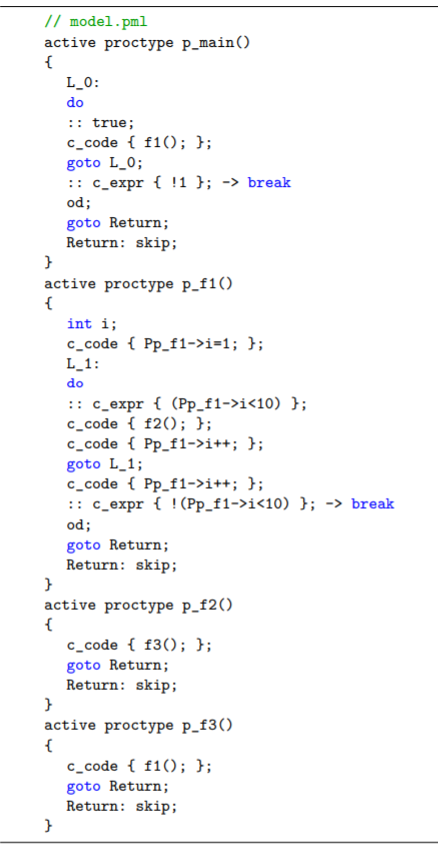
\includegraphics[height=25cm,width=12cm]{g.png}
	\caption{فایل نتیجه Modex}
	\centering
\end{figure}

%\hspace{0.5cm}
%\begin{latin}
%	\begin{lstlisting}
%		// model.pml
%		active proctype p_main()
%		{
%			L_0:
%			do
%			:: true;
%			c_code { f1(); };
%			goto L_0;
%			:: c_expr { !1 }; -> break
%			od;
%			goto Return;
%			Return: skip;
%		}
%		active proctype p_f1()
%		{
%			int i;
%			c_code { Pp_f1->i=1; };
%			L_1:
%			do
%			:: c_expr { (Pp_f1->i<10) };
%			c_code { f2(); };
%			c_code { Pp_f1->i++; };
%			goto L_1;
%			c_code { Pp_f1->i++; };
%			:: c_expr { !(Pp_f1->i<10) }; -> break
%			od;
%			goto Return;
%			Return: skip;
%		}
%		active proctype p_f2()
%		{
%			c_code { f3(); };
%			goto Return;
%			Return: skip;
%		}
%		active proctype p_f3()
%		{
%			c_code { f1(); };
%			goto Return;
%			Return: skip;
%		}
%	\end{lstlisting}
%\end{latin}

در این حالت با توجه به اینکه رویه‌ها از ابتدا فعال هستند، ولی این‌بار با استفاده از کانال‌های هم‌گام‌ساز سعی در کنترل ترتیب اجرای آن‌ها نشده؛ تعداد مسیرهای اجرایی نسبت به حالت قبل هم بیشتر است و همچنان شامل مسیر درست نیست. بنابراین، این حالت نسبت به حالت اول هم عدم قطعیت\LTRfootnote{non-determinism}   بیشتری دارد.


\section{اصلاح مدل خروجی Modex}
هدف این پژوهش اصلاح همین نقص Modex که در بخش 4.2 توصیف شده؛ یعنی عدم توانایی در مدل‌سازی صحیح مدل‌های پیچیده از لحاظ توالی فراخوانی توابع است.
\\
در ادامه سعی می‌شود با ایجاد تغییراتی در کد مدل تولیدی Modex در بخش 4.2.2 ، ترتیب فراخوانی رویه‌های مدل  Promela را منطبق بر توالی اجرای تابع‌ها در کد C کرد.

\subsection{گام اول}
کد حاصل از این گام، به صورت کد نشان داده شده در شکل 4-8 است.

 \begin{figure}
	\centering
	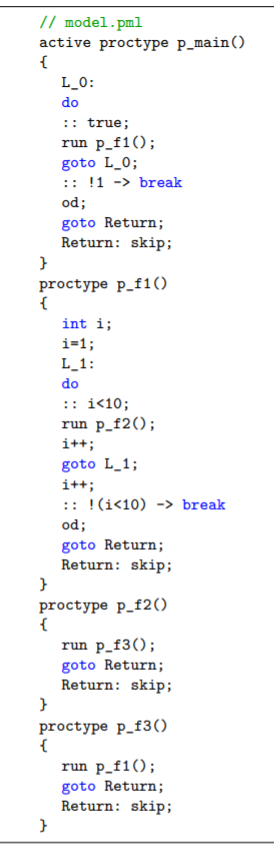
\includegraphics[height=23cm,width=7cm]{h.png}
	\caption{کد حاصل از گام اول}
	\centering
\end{figure}

%\hspace{0.5cm}
%\begin{latin}
%	\begin{lstlisting}
%		// model.pml
%		active proctype p_main()
%		{
%			L_0:
%			do
%			:: true;
%			run p_f1();
%			goto L_0;
%			:: !1 -> break
%			od;
%			goto Return;
%			Return: skip;
%		}
%		proctype p_f1()
%		{
%			int i;
%			i=1;
%			L_1:
%			do
%			:: i<10;
%			run p_f2();
%			i++;
%			goto L_1;
%			i++;
%			:: !(i<10) -> break
%			od;
%			goto Return;
%			Return: skip;
%		}
%		proctype p_f2()
%		{
%			run p_f3();
%			goto Return;
%			Return: skip;
%		}
%		proctype p_f3()
%		{
%			run p_f1();
%			goto Return;
%			Return: skip;
%		}
%	\end{lstlisting}
%\end{latin}

تغییرات ایجاد شده، شامل موارد زیر است:
\begin{enumerate}
	\item قطعه کدهای ساده‌ی مشترک بین دو زبان که در بلاک‌های تعبیه شده‌ی کد C \LTRfootnote{C-expression}    قرار داشت، از این بلاک‌ها خارج شده و به صورت کد Promela در مدل قرار گرفت. به این ترتیب، قابلیت وارسی این بخش از مدل هم توسط Spin فراهم شد.
	\item فقط تابع اصلی برنامه به صورت فعال تعریف شده‌است. بقیه‌ی توابع، در هنگام فراخوانی، با کلیداژه‌ی run اجرا می‌شوند. (برای اصلاح مشکل فراخوانی توابع، نمی‌توان از توابع inline بهره گرفت؛ چرا که در این توابع، ترتیب تعریف بدنه‌ی توابع برای امکان فراخوانی آن‌ها توسط یک‌دیگراهمیت دارد، و این موجب ایجاد محدودیت در تنوع فراخوانی های توابع می‌شود.)
\end{enumerate}

حال برای بررسی این مدل و مسیرهای اجرایی ممکن در آن، از Spin استفاده می‌کنیم.
\\
در این حالت، مشاهده می‌شود که همچنان تعداد مسیرهای اجرایی ممکن، بیش از یک مسیر است. با این حال، بهبودی که در این حالت دیده می‌شود، این است که ترتیب اجرای رویه‌ها در یکی از مسیرهای اجرایی، منطبق بر ترتیب اجرای توابع در کد C متناظر است. یعنی مدل Promela تهیه شده، علاوه بر رفتار مدل اصلی C ، رفتارهای دیگری هم از خود نشان‌ می‌دهد. در این حالت اگر به این کد  Promla به عنوان نماینده‌ی کد C مورد نظر و برای بررسی آن با استفاده از Spin تکیه کنیم، نتیجه می‌گیریم که مدل ما همواره رفتار موردنظر ما را ندارد. این نتیجه‌گیری نادرست، به دلیل وجود همان مسیرهای غیر از مسیر اصلی و درست کد C است. در این حالت اصطلاحاً گفته می‌شود که این نتیجه، منفی کاذب \LTRfootnote{false negative}    است.
\\
این مشکل به دلیل این است که وقتی یک رویه، رویه‌ی دیگری را فراخوانی می‌کند، هم خود رویه‌ی اول و هم رویه‌ی فراخوانی شده، امکان اجرا دارند. در این حالت، اطمینانی وجود ندارد که بدنه‌ی کدام‌یک از این دو تابع اجرا خواهدشد. و این قضیه موجب ایجاد عدم قطعیت در رفتار مدل می‌شود. پس باید مسیر اجرای یکی از این دو رویه بلاک شود، تا مسیر مورد انتظار اجرا شود.
\\
مسیر موردانتظار که در مسیرهای اجرایی این مدل وجود دارد، به صورت شکل 4-9 است.

 \begin{figure}
	\centering
	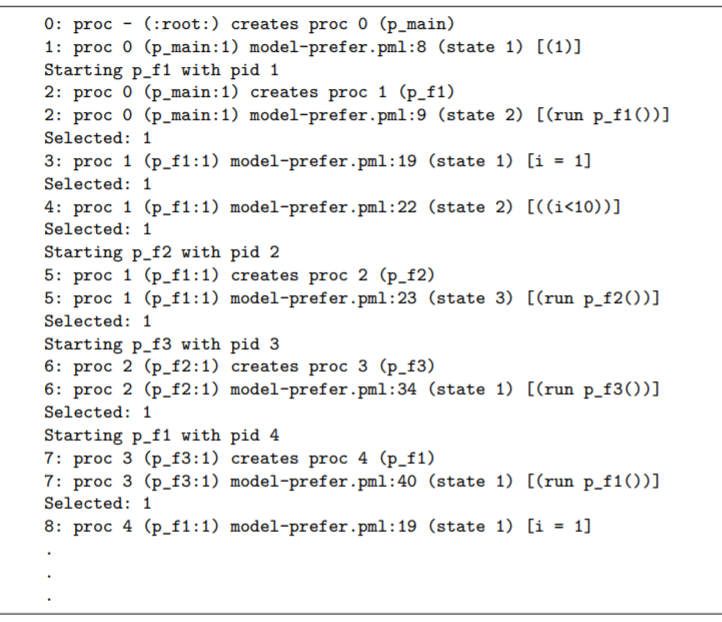
\includegraphics[height=10cm,width=15cm]{i.png}
	\caption{مسیر اجرایی مربوط به کد حاصل از گام اول}
	\centering
\end{figure}

%\hspace{0.5cm}
%\begin{latin}
%	\begin{lstlisting}
%		0:	proc  - (:root:) creates proc  0 (p_main)
%		1:	proc  0 (p_main:1) model-prefer.pml:8 (state 1)	[(1)]
%		Starting p_f1 with pid 1
%		2:	proc  0 (p_main:1) creates proc  1 (p_f1)
%		2:	proc  0 (p_main:1) model-prefer.pml:9 (state 2)	[(run p_f1())]
%		Selected: 1
%		3:	proc  1 (p_f1:1) model-prefer.pml:19 (state 1)	[i = 1]
%		Selected: 1
%		4:	proc  1 (p_f1:1) model-prefer.pml:22 (state 2)	[((i<10))]
%		Selected: 1
%		Starting p_f2 with pid 2
%		5:	proc  1 (p_f1:1) creates proc  2 (p_f2)
%		5:	proc  1 (p_f1:1) model-prefer.pml:23 (state 3)	[(run p_f2())]
%		Selected: 1
%		Starting p_f3 with pid 3
%		6:	proc  2 (p_f2:1) creates proc  3 (p_f3)
%		6:	proc  2 (p_f2:1) model-prefer.pml:34 (state 1)	[(run p_f3())]
%		Selected: 1
%		Starting p_f1 with pid 4
%		7:	proc  3 (p_f3:1) creates proc  4 (p_f1)
%		7:	proc  3 (p_f3:1) model-prefer.pml:40 (state 1)	[(run p_f1())]
%		Selected: 1
%		8:	proc  4 (p_f1:1) model-prefer.pml:19 (state 1)	[i = 1]
%		.
%		.
%		.
%	\end{lstlisting}
%\end{latin}

\subsection{گام دوم}
کد حاصل از این گام، به صورت کد نشان داده شده در دو شکل 4-10 و 4-11 است.

\begin{figure}
	\centering
	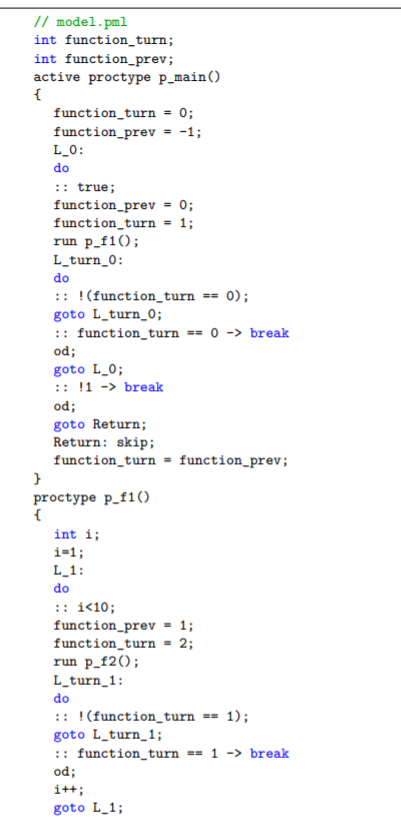
\includegraphics[height=23cm,width=10cm]{j1.png}
	\caption{کد حاصل از گام دوم}
	\centering
\end{figure}

\begin{figure}
	\centering
	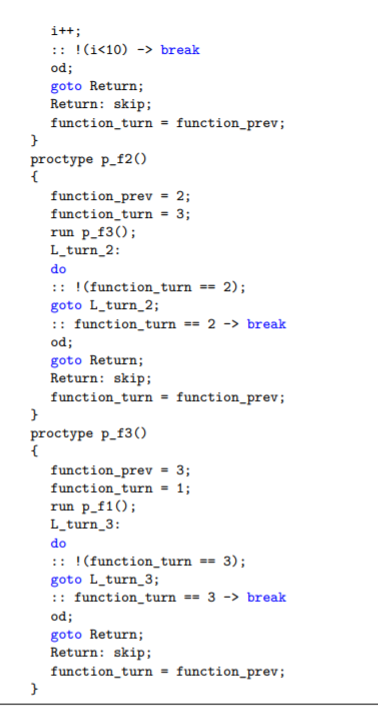
\includegraphics[height=23cm,width=11cm]{j2.png}
	\caption{ادامه کد حاصل از گام دوم}
	\centering
\end{figure}


%\hspace{0.5cm}
%\begin{latin}
%	\begin{lstlisting}
%		// model.pml
%		int function_turn;
%		int function_prev;
%		active proctype p_main()
%		{
%			function_turn = 0;
%			function_prev = -1;
%			L_0:
%			do
%			:: true;
%			function_prev = 0;
%			function_turn = 1;
%			run p_f1();
%			L_turn_0:
%			do
%			:: !(function_turn == 0);
%			goto L_turn_0;
%			:: function_turn == 0 -> break
%			od; 
%			goto L_0;
%			:: !1 -> break
%			od;
%			goto Return;
%			Return: skip;
%			function_turn = function_prev;
%		}
%		proctype p_f1()
%		{
%			int i;
%			i=1;
%			L_1:
%			do
%			:: i<10;
%			function_prev = 1;
%			function_turn = 2;
%			run p_f2();
%			L_turn_1:
%			do
%			:: !(function_turn == 1);
%			goto L_turn_1;
%			:: function_turn == 1 -> break
%			od; 
%			i++;
%			goto L_1;
%			i++;
%			:: !(i<10) -> break
%			od;
%			goto Return;
%			Return: skip;
%			function_turn = function_prev;
%		}
%		proctype p_f2()
%		{
%			function_prev = 2;
%			function_turn = 3;
%			run p_f3();
%			L_turn_2:
%			do
%			:: !(function_turn == 2);
%			goto L_turn_2;
%			:: function_turn == 2 -> break
%			od; 
%			goto Return;
%			Return: skip;
%			function_turn = function_prev;
%		}
%		proctype p_f3()
%		{
%			function_prev = 3;
%			function_turn = 1;
%			run p_f1();
%			L_turn_3:
%			do
%			:: !(function_turn == 3);
%			goto L_turn_3;
%			:: function_turn == 3 -> break
%			od; 
%			goto Return;
%			Return: skip;
%			function_turn = function_prev;
%		}
%	\end{lstlisting}
%\end{latin}

دراین گام سعی شد تا با تعریف دو متغیر عمومی\LTRfootnote{global variables}، در هنگامی که بدنه‌ی چند رویه به صورت هم‌زمان امکان اجرا داشتند، رویه‌هایی که موجب مسیر غیرمنتظره می‌‍شوند بلاک شود. یکی از متغیرها به منظور نشان دادن این است که رویه‌ای که باید اجرا شود، کدام است\LTRfootnote{function turn}. متغیر دیگر این را نشان می‌دهد که اگر رویه‌ای که در حال حاضر در آن قرار داریم به اتمام رسید، کدام رویه باید اجرا شود(با توجه به اینکه رویه‌ی حال حاضر توسط چه رویه‌ای فراخوانی شده است، تنظیم می‌شود) \LTRfootnote{function prev}.
\\
در این حالت، همچنان دو مشکل وجود دارد:
\begin{enumerate}
	\item دراین حالت، با استفاده از یک حلقه‌ سعی شده در هر رویه چک شود که آیا می‌تواند به اجرای بدنه‌ی خود ادامه دهد، یا بلاک شود. برای مثال وقتی که یک رویه، رویه‌ی دیگری را فراخوانی می‌کند، پس از آن باید وارد حلقه شود و به طور مرتب چک کند که آیا می‌تواند به اجرای بدنه‌ی خود ادامه بدهد یا خیر. اینجا مشکلی که پیش می‌آید، این است که ممکن است تمام cpu به رویه‌ی اول اختصاص پیدا کند و رویه‌ی دوم نتواند هیچ‌وقت اجرا شود. بنابراین، همچنان قطعیتی روی مسیر اجرای برنامه وجود ندارد، و مشخص نیست بدنه‌ی کدام رویه پس از آن اجرا می‌شود.
	\item مشکل دیگر، مربوط به کنترل مسیر اجرا با استفاده از متغیرهای عمومی به کارگرفته شده‌است. در این حالت، هر رویه اگر بیش از یک بار به روش های مختلف قصد اجرا داشته باشد، این متغیرها کارایی خود را از دست می‌دهند و به درستی ترتیب اجرای رویه‎‌ها را نمی‌توانند کنترل کنند. برای مثال اگر در تابع 1، تابع 2 فراحوانی شد، بدنه‌ی تابع 1 روی خط بعد از فراخوانی تابع 2 باید بلاک شود. حالا اگر دوباره از طریق تابع 2، تابع 1 فراخوانی شود، تابع 1 هم از ابتدا می‌تواند اجرا شود و هم از خطی که در میانه‌ ی بدنه‌اش بلاک شده بود؛ درحالی که ما انتظار داشتیم تابع 1 فقط از ابتدا اجرا شود و نمونه ی اولیه‌ی آن همچنان در بدنه‌ی خود بلاک بماند تا آن نمونه از تابع 1 که اجرا کرده‌بود، به اتمام برسد.
\end{enumerate}

\subsection{گام سوم}
کد حاصل از این گام، به صورت کد نشان داده شده در شکل 4-12 است.

\begin{figure}
	\centering
	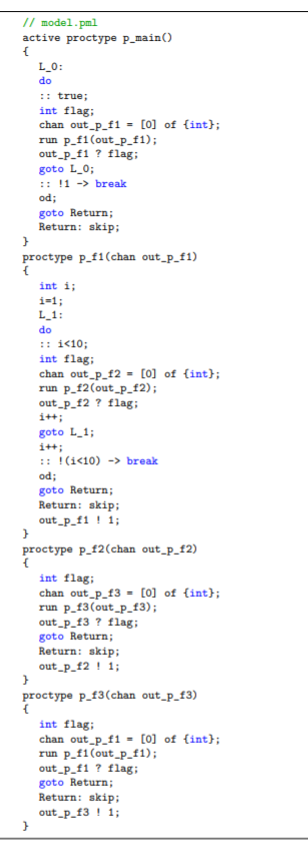
\includegraphics[height=23cm,width=9cm]{k.png}
	\caption{کد حاصل از گام سوم}
	\centering
\end{figure}


%\hspace{0.5cm}
%\begin{latin}
%	\begin{lstlisting}
%		// model.pml
%		active proctype p_main()
%		{
%			L_0:
%			do
%			:: true;
%			int flag;
%			chan out_p_f1 = [0] of {int};
%			run p_f1(out_p_f1);
%			out_p_f1 ? flag;
%			goto L_0;
%			:: !1 -> break
%			od;
%			goto Return;
%			Return: skip;
%		}
%		proctype p_f1(chan out_p_f1)
%		{
%			int i;
%			i=1;
%			L_1:
%			do
%			:: i<10;
%			int flag;
%			chan out_p_f2 = [0] of {int};
%			run p_f2(out_p_f2);
%			out_p_f2 ? flag;
%			i++;
%			goto L_1;
%			i++;
%			:: !(i<10) -> break
%			od;
%			goto Return;
%			Return: skip;
%			out_p_f1 ! 1;
%		}
%		proctype p_f2(chan out_p_f2)
%		{
%			int flag;
%			chan out_p_f3 = [0] of {int};
%			run p_f3(out_p_f3);
%			out_p_f3 ? flag;
%			goto Return;
%			Return: skip;
%			out_p_f2 ! 1;
%		}
%		proctype p_f3(chan out_p_f3)
%		{
%			int flag;
%			chan out_p_f1 = [0] of {int};
%			run p_f1(out_p_f1);
%			out_p_f1 ? flag;
%			goto Return;
%			Return: skip;
%			out_p_f3 ! 1;
%		}
%	\end{lstlisting}
%\end{latin}
در این حالت، برای کنترل ترتیب اجرای رویه‌ها، به جای استفاده از متغیرهای عمومی، از کانال‌های هم‌گام‌ساز محلی\LTRfootnote{local synchronization channels} استفاده می‌شود. به این ترتیب، هر دو مشکلی که در گام قبل با آن‌ها مواجه بودیم، برطرف می‌شود. روش استفاده از این کانال‌ها به این صورت است که در هر فراخوانی رویه، یک کانال هم‌گام‌ساز بین دو رویه فراخوانی‌کننده و فراخوانی‌شونده تنظیم می‌شود، تا اجرای این دو رویه را کنترل کند. به این ترتیب، با توجه به اینکه در هر فراخوانی رویه، یک کانال جداگانه بین نمونه‌های رویه‌ها تنظیم می‌شود، مشکل دوم گام قبل حل می‌شود. همچنین، در بدنه‌ی رویه فراخوانی‌کننده، در خط پس از خط فراخوانی، منتظر دریافت مقدار از طریق کانال می‌ماند و در همان خط بلاک می‌شود و نیاز به اختصاص مرتب cpu  نخواهدداشت و عدم قطعیتی در مسیر اجرا ایجاد نمی‌کند.
\\
تنها مسیر اجرای حاصل از مدل در این گام، که همان مسیر درست است، در شکل 4-13 نشان ‌داده‌شده‌‍است.

\begin{figure}
	\centering
	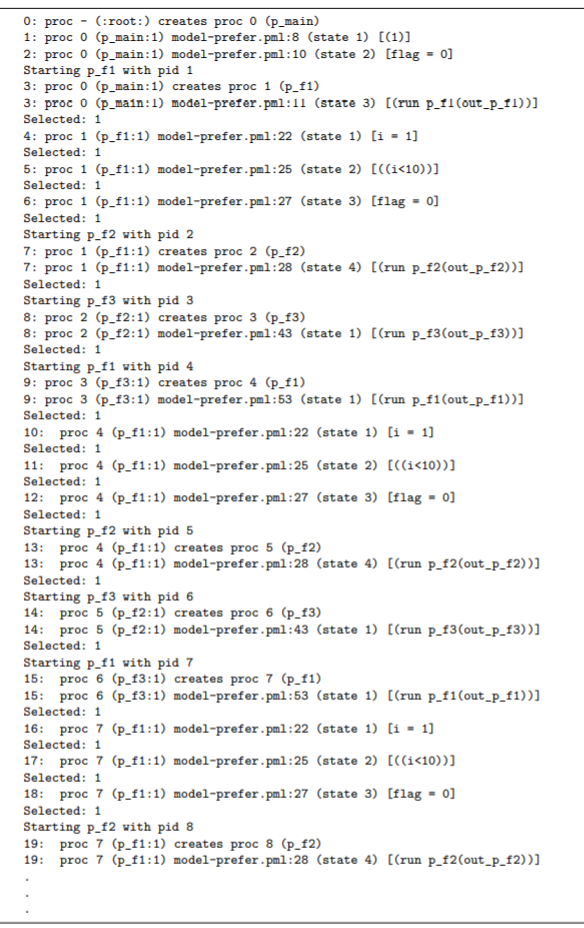
\includegraphics[height=23cm,width=12cm]{l.png}
	\caption{مسیر اجرایی مربوط به کد حاصل از گام سوم}
	\centering
\end{figure}


%\hspace{0.5cm}
%\begin{latin}
%	\begin{lstlisting}
%		0:	proc  - (:root:) creates proc  0 (p_main)
%		1:	proc  0 (p_main:1) model-prefer.pml:8 (state 1)	[(1)]
%		2:	proc  0 (p_main:1) model-prefer.pml:10 (state 2)	[flag = 0]
%		Starting p_f1 with pid 1
%		3:	proc  0 (p_main:1) creates proc  1 (p_f1)
%		3:	proc  0 (p_main:1) model-prefer.pml:11 (state 3)	[(run p_f1(out_p_f1))]
%		Selected: 1
%		4:	proc  1 (p_f1:1) model-prefer.pml:22 (state 1)	[i = 1]
%		Selected: 1
%		5:	proc  1 (p_f1:1) model-prefer.pml:25 (state 2)	[((i<10))]
%		Selected: 1
%		6:	proc  1 (p_f1:1) model-prefer.pml:27 (state 3)	[flag = 0]
%		Selected: 1
%		Starting p_f2 with pid 2
%		7:	proc  1 (p_f1:1) creates proc  2 (p_f2)
%		7:	proc  1 (p_f1:1) model-prefer.pml:28 (state 4)	[(run p_f2(out_p_f2))]
%		Selected: 1
%		Starting p_f3 with pid 3
%		8:	proc  2 (p_f2:1) creates proc  3 (p_f3)
%		8:	proc  2 (p_f2:1) model-prefer.pml:43 (state 1)	[(run p_f3(out_p_f3))]
%		Selected: 1
%		Starting p_f1 with pid 4
%		9:	proc  3 (p_f3:1) creates proc  4 (p_f1)
%		9:	proc  3 (p_f3:1) model-prefer.pml:53 (state 1)	[(run p_f1(out_p_f1))]
%		Selected: 1
%		10:	proc  4 (p_f1:1) model-prefer.pml:22 (state 1)	[i = 1]
%		Selected: 1
%		11:	proc  4 (p_f1:1) model-prefer.pml:25 (state 2)	[((i<10))]
%		Selected: 1
%		12:	proc  4 (p_f1:1) model-prefer.pml:27 (state 3)	[flag = 0]
%		Selected: 1
%		Starting p_f2 with pid 5
%		13:	proc  4 (p_f1:1) creates proc  5 (p_f2)
%		13:	proc  4 (p_f1:1) model-prefer.pml:28 (state 4)	[(run p_f2(out_p_f2))]
%		Selected: 1
%		Starting p_f3 with pid 6
%		14:	proc  5 (p_f2:1) creates proc  6 (p_f3)
%		14:	proc  5 (p_f2:1) model-prefer.pml:43 (state 1)	[(run p_f3(out_p_f3))]
%		Selected: 1
%		Starting p_f1 with pid 7
%		15:	proc  6 (p_f3:1) creates proc  7 (p_f1)
%		15:	proc  6 (p_f3:1) model-prefer.pml:53 (state 1)	[(run p_f1(out_p_f1))]
%		Selected: 1
%		16:	proc  7 (p_f1:1) model-prefer.pml:22 (state 1)	[i = 1]
%		Selected: 1
%		17:	proc  7 (p_f1:1) model-prefer.pml:25 (state 2)	[((i<10))]
%		Selected: 1
%		18:	proc  7 (p_f1:1) model-prefer.pml:27 (state 3)	[flag = 0]
%		Selected: 1
%		Starting p_f2 with pid 8
%		19:	proc  7 (p_f1:1) creates proc  8 (p_f2)
%		19:	proc  7 (p_f1:1) model-prefer.pml:28 (state 4)	[(run p_f2(out_p_f2))]
%		.
%		.
%		.
%	\end{lstlisting}
%\end{latin}